%\documentclass[9pt]{scrartcl}
\documentclass[a4paper]{article}
\usepackage[]{amsmath}
\usepackage{tikz}
\usetikzlibrary{positioning}
%\usepackage{helvet}
\usepackage{listings}
\usepackage{geometry}
%\geometry{textheight=\paperheight, noheadfoot, nomarginpar}
\usetikzlibrary{positioning,shapes,shadows}
\renewcommand{\familydefault}{\sfdefault}

\tikzstyle{abstract}=[rectangle, draw=black, fill=gray!20, text centered,  text=black, text width=12.5mm]
\tikzstyle{spacestyle}=[rectangle, draw=black, fill=gray!20, text centered,  text=black, text width=50mm]

\lstset{
        language=python,
        basicstyle=\fontencoding{T1}\ttfamily,
        commentstyle=\color{gray},
        keywordstyle=\color{OliveGreen},
        frame=single,
        backgroundcolor=\color{lightlightgray},
        tabsize=2,
        %deletestring=[d]",
        %escapechar=\%,
        numbers=left,
        showstringspaces=false,
}
\usepackage[explicit]{titlesec} 
\titleformat{\section}{\normalfont\Large\bfseries}{}{0em}{#1}
\titleformat{\subsection}{\normalfont\bfseries}{}{0em}{--#1}

\newcommand{\arrow}[4]{%
\draw[-latex, thick,#4] ([yshift=-0.6 *\they cm-0.5  cm] #1.south) -- ([yshift=-0.6*\they cm-0.9 cm] #2.south) node[midway,above right] {#3};%
} 
\newcommand{\arrowred}[3]{%
\draw[-latex, thick, red] ([yshift=-0.6 *\they cm-0.5  cm] #1.south) -- ([yshift=-0.6*\they cm-0.9 cm] #2.south) node[midway,above right] {#3};%
} 
\newcommand{\arrowfar}[4]{%
\draw[-latex, thick, #4] ([yshift=-0.6 *\they cm-0.5  cm] #1.south) -- ([yshift=-0.6*\they cm-1.5 cm] #2.south) node[midway,above right] {#3};%
} 
\newcommand{\arrowredfar}[3]{%
\draw[-latex, thick,red] ([yshift=-0.6 *\they cm-0.5  cm] #1.south) -- ([yshift=-0.6*\they cm-1.5 cm] #2.south) node[midway,above right] {#3};%
} 

\newcommand{\mykey}[2]{%
\begin{tikzpicture} \node (Item) [abstract, minimum size=12.5mm, align=center]
{\vrule height 12pt depth 8pt width 0pt\textbf{#1} \\\vrule height 6pt depth 8pt width 0pt\parbox{1.25cm}{\centering{\fontsize{6pt}{8pt}\selectfont{#2}}}};%
\end{tikzpicture}}


\begin{document}
\begin{center}
\Large{Diagram}
\end{center}
\noindent%


\section {Two-phase commit protocol (2PC)}

Successful transactions\\\\
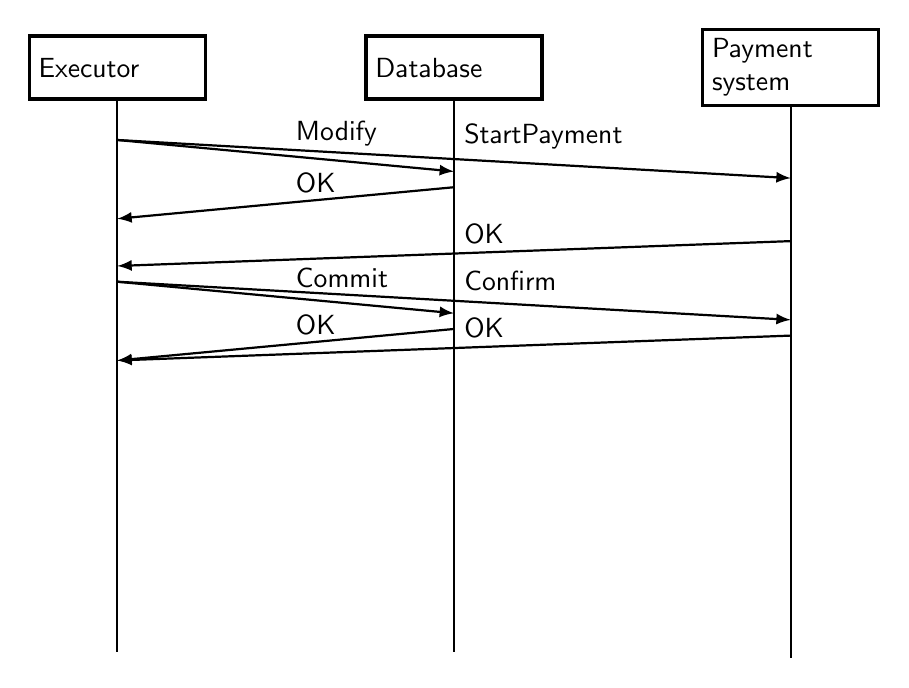
\begin{tikzpicture}

% Client
\node [draw,
	minimum width=2cm,
	minimum height=0.8cm,
	text width=2cm,
	very thick,
]  (client) {
Executor
};

% Database 1
\node [draw,
	minimum width=2cm,
	minimum height=0.8cm,
	text width=2cm,
	very thick,
	right = 2cm of client
]  (db) {
Database
};
% Database 2
\node [draw,
	minimum width=2cm,
	minimum height=0.8cm,
	text width=2cm,
	very thick,
	right = 2cm of db
]  (ps) {
Payment\\system
};


% Arrows with text label

\draw[thick] (client.south) -- ([yshift=-7cm] client.south);
\draw[thick] (db.south) -- ([yshift=-7cm] db.south);
\draw[thick] (ps.south) -- ([yshift=-7cm] ps.south);
%\draw[very thick,red] ([yshift=-1.6cm]ps.south) -- ([yshift=-4cm] ps.south);
%\draw[very thick,red] ([yshift=-1cm]db.south) -- ([yshift=-4.6cm] db.south);

\newcounter{y}
\arrow{client}{db}{Modify}{black}
\arrow{client}{ps}{StartPayment}{black}
\stepcounter{y};

\arrow{db}{client}{OK}{black}
\stepcounter{y};
\arrow{ps}{client}{OK}{black}
\stepcounter{y};

\arrow{client}{db}{Commit}{black}
\arrow{client}{ps}{Confirm}{black}
\stepcounter{y};
\arrow{ps}{client}{OK}{black}
\arrow{db}{client}{OK}{black}


\end{tikzpicture}

\pagebreak
\noindent
Failing transactions\\\\
\begin{tikzpicture}

% Client
\node [draw,
	minimum width=2cm,
	minimum height=0.8cm,
	text width=2cm,
	very thick,
]  (client) {
Executor
};

% Database 1
\node [draw,
	minimum width=2cm,
	minimum height=0.8cm,
	text width=2cm,
	very thick,
	right = 2cm of client
]  (db) {
Database
};
% Database 2
\node [draw,
	minimum width=2cm,
	minimum height=0.8cm,
	text width=2cm,
	very thick,
	right = 2cm of db
]  (ps) {
Payment\\system
};


% Arrows with text label

\draw[thick] (client.south) -- ([yshift=-7cm] client.south);
\draw[thick] (db.south) -- ([yshift=-7cm] db.south);
\draw[thick] (ps.south) -- ([yshift=-7cm] ps.south);
%\draw[very thick,red] ([yshift=-1.6cm]ps.south) -- ([yshift=-4cm] ps.south);
%\draw[very thick,red] ([yshift=-1cm]db.south) -- ([yshift=-4.6cm] db.south);

\setcounter{y}0
\arrow{client}{db}{Modify}{black}
\arrow{client}{ps}{StartPayment}{black}
\stepcounter{y};

\arrow{db}{client}{OK}{black}
\stepcounter{y};
\arrow{ps}{client}{Fail}{black}
\stepcounter{y};

\arrow{client}{db}{Abort}{black}
\arrow{client}{ps}{Abort}{black}
\stepcounter{y};
\arrow{ps}{client}{OK}{black}
\arrow{db}{client}{OK}{black}


\end{tikzpicture}


\end{document}